\documentclass{article}
\usepackage{tikz,times}
\usepackage[paperwidth=23cm,paperheight=16cm,left=1cm,top=1cm]{geometry}

\usetikzlibrary{mindmap,backgrounds}

\pagestyle{empty}

\begin{document}
\centering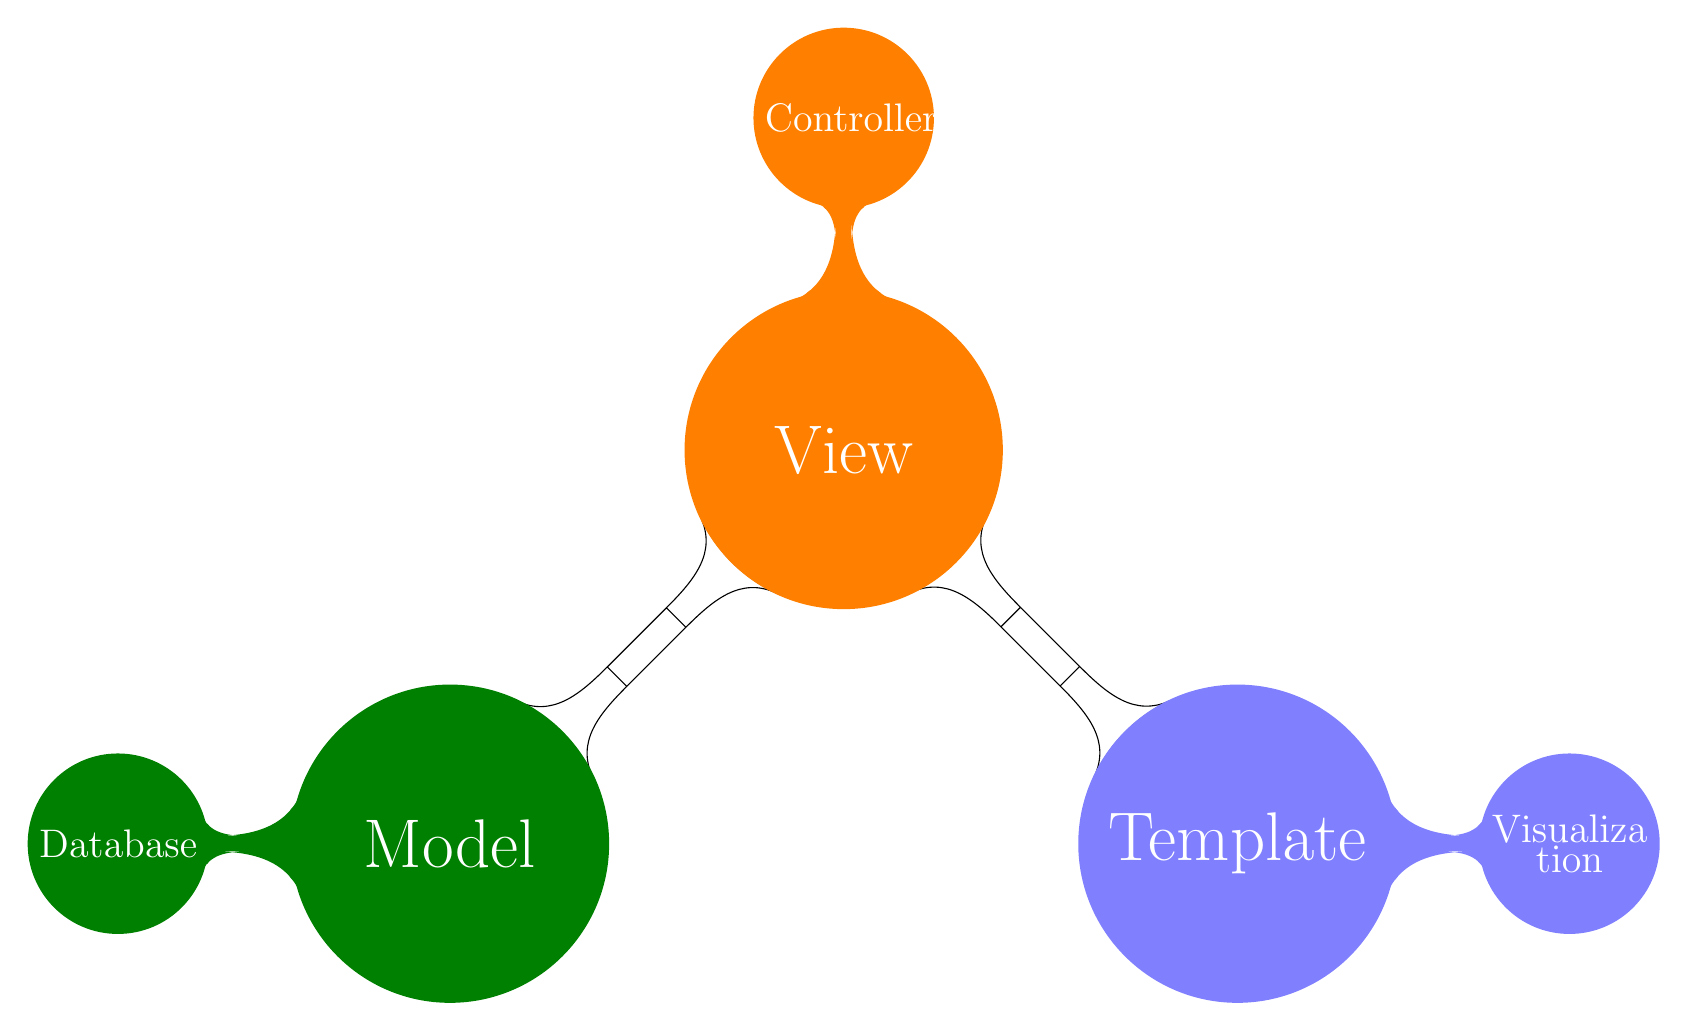
\begin{tikzpicture}[mindmap,
  level 1 concept/.append style={level distance=130,sibling angle=30},
  extra concept/.append style={color=blue!50,text=black}]


  \begin{scope}[mindmap, concept color=orange,text=white]
    \node [concept] (v) at (0,0) {\Huge View}
      child [concept color=orange, grow=90, level distance=120] 
        {node [concept] {\Large Controller}};
  \end{scope}

  \begin{scope}[mindmap, concept color=green!50!black,text=white]
    \node [concept] (m) at (-5,-5) {\Huge Model}
      child [concept color=green!50!black, grow=180, level distance=120] 
        {node [concept] {\Large Database}};
  \end{scope}

  \begin{scope}[mindmap, concept color=blue!50,text=white]
    \node [concept] (t) at (5,-5) {\Huge Template}
      child [concept color=blue!50, grow=0, level distance=120] 
        {node [concept] {\Large Visualiza\ tion}};
  \end{scope}

  \begin{pgfonlayer}{background}
    \draw [circle connection bar]
      (m) edge (v)
      (v) edge (t);
  \end{pgfonlayer}
\end{tikzpicture}

\end{document}